% TODO:
%   o Rose mentions centrality; important for us?

\section{Introduction}

%% Don't forget:
%% - Mention control charts as real-time tools. Snippet at end.
%% Points to make:
%% - Why forum important
%%     o For humanities
%%     o For helping each other
%% - Not all participate
%%     o why?
%%     o Observing actions every week to predict dropout.
%%       Maybe had forum actions?:
%%       Balakrishnan Girish. Predicting Student Retention in Massive
%%       Open Online Courses using Hidden MarkovModels. EECS Department,
%%       University of California, Berkeley, May, 2013.   

%% - Residential is different from MOOCs:
%%     o Incentives: more at stake after drop-out
%%     o Problem of forum cliques falling apart from
%%       course attrition goes away.
%%     o No late-comers that stay at the periphery
%%         (Rose:Turn-off)
%%     o Possible prior acquaintance
%%     o Smaller
%% - We have evidence that encouragement tricky
%%     o Grade: reduces intrinsic motivation.
%%     o Appeal to personal growth: negative
%%     o Appeal to community ?
%%     o These interventions were at the start, when
%%         urgency not there yet.
%% - Now: many courses available: reruns and varied
%%     o We can see dynamics of forum participation
%%       over time through a course. For top and
%%       average students.
%%     o When do prolific students tend to get engaged?
%%     o At any point in time, can we see a
%%       trajectory of prolific and median students?

%% - Analyzed the graph, snapshots over time. Are there
%%   inflection points?

%%     o Cite
%%       [14] Borgatti, Stephen P. Centrality and network flow. Social
%%       networks 27.1 (2005): 55-71. Rose uses their interpretation of
%%       what the social graphs mean 
%%     o Identify places where encouragement could be given.
%%       Inflection points?

%%     o We don't discuss the *form* of encouragement, though
%%       the messaging is important:

%%       * These say that emotional support is important:

%%         [13] Wang, Yi-Chia, Robert Kraut, and John M. Levine. To stay
%%         or leave?: the relationship of emotionaland informational support
%%         to commitment in online health support groups. Proceedings of the
%%         ACM 2012conference on Computer Supported Cooperative Work. ACM,
%%         2012.       
%%       * Could appeal to personal gain for forum participation,
%%       * Could appeal to community gain for forum participation,
%%       * Could just state facts.

\section{Introduction}

Many massively open online course (MOOCs) rely heavily on online forum
facilities. The remote course participants are expected to communicate
by posting questions and opinions on the learning management system's
forum. Instructors and teaching assistants sometimes selectively
respond via that medium. Importantly, the courses rely on the students
themselves to answer each others' questions in comments to
posts. Whereas in science courses the forum often serves primarily the
exchange of questions and answers, humanities courses frequently
require discussions among students. The forum plays an even more
central part in these scenarios.

Given their importance in MOOCs, a number of studies have examined
student behaviors on forum facilities. For example, forum
participation has been studies as an early indicator of student
dropout \cite{yang2013}. The distribution of forum post submissions
among course participants was examined in \cite{Huang2014}. This
examination showed the frequent posters, or {\em superposters} do
better in courses than the average of other participants. The authors
further find that the presence of superposters has positive impact on
the rest of the forum participants.

Maybe related to the by necessity heavy reliance on forum
communication in MOOCs, forum facilities have also steadily gained
acceptance in residential, classroom bound courses. The forum there is
a supplement to in-class discussion---if such face-to-face
interactions even occur. Studies on how academic outcomes are related
to forum participation in residential settings are missing because
access to grades in these settings tends to be highly restricted.

However, we can at least hypothesize that benefits such as those found
by \cite{Huang2014} do carry over to residential students. If we
accept for the moment that forum participation is indeed beneficial,
then we can ask how to encourage students to participate with posts
and comments on others' contributions.


\section{Dataset}

Since 2011 many courses in the university have used the Piazza forum
facility for its internal courses. Our dataset comprises the posts and
comments of these usage years. From among 5000 university course
offerings that have used the Piazza forum facility since 2011 we
selected **** courses, with a total of **** offerings. Most courses
were taught multiple times since 2011, so we include longitudinal
forum usage data for most courses. One course was taught as a MOOC,
and used Piazza; we included that data for comparison. Most MOOCs make
use of the delivery platform's built-in forum facility.

We used two criteria for selecting the courses to analyze. We favored
those that had comparatively large numbers of student posts, and we
tried to cover courses from many schools and departments. We in
particular sought to include Humanities courses that made use of
 Piazza for class discussion. Table~\ref{tab:simpleCrsStats} summarizes
 our choice.
 
 \begin{figure}[htp]
       \centering
       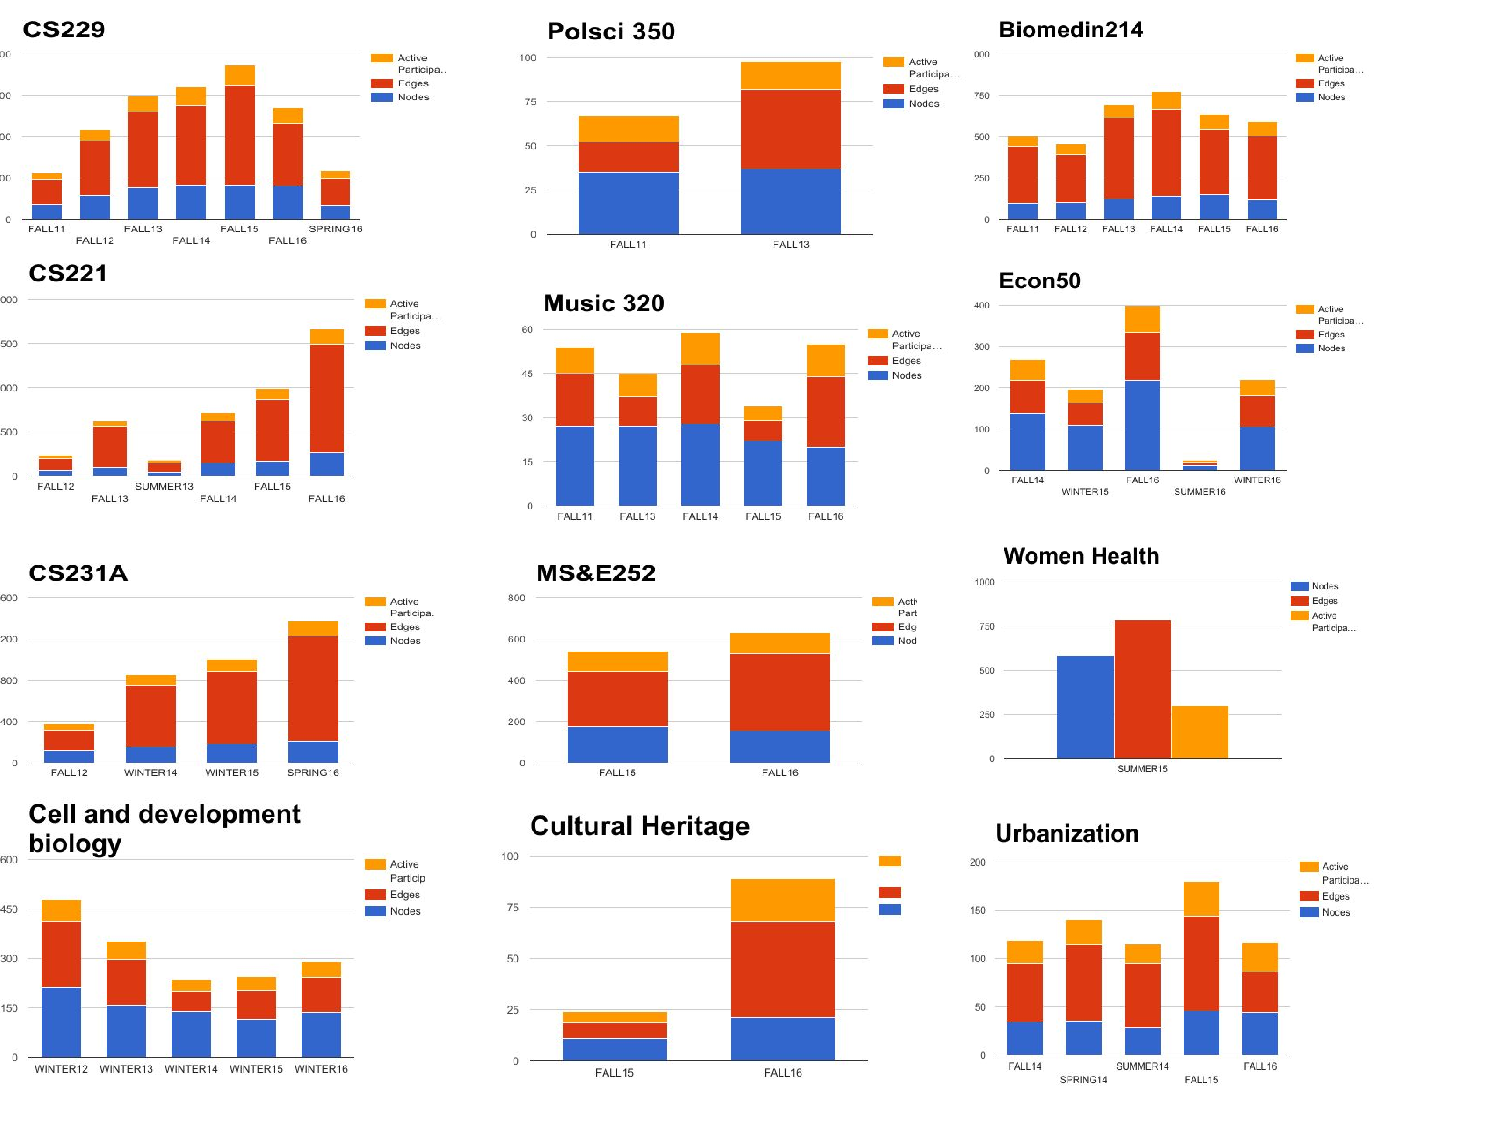
\includegraphics[width=1.2\textwidth]{Figs/nodes2.pdf}
       \caption{\textnormal{Number of users, active users and their degrees}}
       \label{fig:graphExpl}
\end{figure}
 
 
% \begin{table}[]
% \centering
% \caption{Summary of Courses Used for Analysis}
% \label{tab:simpleCrseStats}
% \begin{tabular}{lllll}
% \multicolumn{1}{c}{\textbf{Course}}                                                  & \multicolumn{1}{c}{\textbf{Offering}} & \multicolumn{1}{c}{\textbf{\begin{tabular}[c]{@{}c@{}}Number of\\ students\end{tabular}}} & \multicolumn{1}{c}{\textbf{\begin{tabular}[c]{@{}c@{}}Students\\ with posts\end{tabular}}} & \multicolumn{1}{c}{\textbf{\begin{tabular}[c]{@{}c@{}}Percentage\\ forum participation\end{tabular}}} \\
% \textbf{\begin{tabular}[c]{@{}l@{}}Artificial\\   Intelligence\end{tabular}}         & FALL12                                & 192                                                                                       & 106                                                                                        & 55\%                                                                                                  \\
% \textbf{}                                                                            & FALL13                                & 278                                                                                       & 195                                                                                        & 70\%                                                                                                  \\
% \textbf{}                                                                            & FALL14                                & 435                                                                                       & 291                                                                                        & 67\%                                                                                                  \\
% \textbf{}                                                                            & FALL15                                & 494                                                                                       & 357                                                                                        & 72\%                                                                                                  \\
% \textbf{}                                                                            & FALL16                                & 782                                                                                       & 529                                                                                        & 68\%                                                                                                  \\
% \textbf{}                                                                            & SUMMER13                              & 137                                                                                       & 81                                                                                         & 59\%                                                                                                  \\
% \textbf{Machine Learning}                                                            & FALL11                                & 356                                                                                       & 166                                                                                        & 47\%                                                                                                  \\
% \textbf{}                                                                            & FALL12                                & 581                                                                                       & 283                                                                                        & 49\%                                                                                                  \\
% \textbf{}                                                                            & FALL13                                & 776                                                                                       & 383                                                                                        & 49\%                                                                                                  \\
% \textbf{}                                                                            & FALL14                                & 820                                                                                       & 449                                                                                        & 55\%                                                                                                  \\
% \textbf{}                                                                            & FALL15                                & 827                                                                                       & 489                                                                                        & 59\%                                                                                                  \\
% \textbf{}                                                                            & FALL16                                & 803                                                                                       & 393                                                                                        & 49\%                                                                                                  \\
% \textbf{}                                                                            & SPRING16                              & 331                                                                                       & 189                                                                                        & 57\%                                                                                                  \\
% \textbf{Computer Vision}                                                             & FALL11                                & 59                                                                                        & 29                                                                                         & 49\%                                                                                                  \\
% \textbf{}                                                                            & FALL12                                & 120                                                                                       & 62                                                                                         & 52\%                                                                                                  \\
% \textbf{}                                                                            & SPRING16                              & 208                                                                                       & 150                                                                                        & 72\%                                                                                                  \\
% \textbf{}                                                                            & WINTER14                              & 152                                                                                       & 101                                                                                        & 66\%                                                                                                  \\
% \textbf{}                                                                            & WINTER15                              & 180                                                                                       & 125                                                                                        & 69\%                                                                                                  \\
% \textbf{Decision Analysis}                                                           & FALL15                                & 176                                                                                       & 100                                                                                        & 57\%                                                                                                  \\
% \textbf{}                                                                            & FALL16                                & 156                                                                                       & 104                                                                                        & 67\%                                                                                                  \\
% \textbf{\begin{tabular}[c]{@{}l@{}}Computational Molecular\\   Biology\end{tabular}} & FALL11                                & 96                                                                                        & 61                                                                                         & 64\%                                                                                                  \\
% \textbf{}                                                                            & FALL12                                & 101                                                                                       & 67                                                                                         & 66\%                                                                                                  \\
% \textbf{}                                                                            & FALL13                                & 123                                                                                       & 80                                                                                         & 65\%                                                                                                  \\
% \textbf{}                                                                            & FALL14                                & 140                                                                                       & 103                                                                                        & 74\%                                                                                                  \\
% \textbf{}                                                                            & FALL15                                & 147                                                                                       & 93                                                                                         & 63\%                                                                                                  \\
% \textbf{}                                                                            & FALL16                                & 120                                                                                       & 86                                                                                         & 72\%                                                                                                 
% \end{tabular}
% \end{table}

From the forum posts of these data we constructed one social graph for
each course offering.

\section{From Posts to Connection Graph}

Social networks are most simply modeled by considering each
participant as a node, and interactions initiated by participants as
out-directed links. In this case all nodes are of one type, and links
are unidirectional. Multiple interaction initiations by one person are
captured by weighting the corresponding outgoing links. Many graph
analysis tools operate on models of this type, and this is the
approach we chose.

However, other strategies exist to cover different goals. For example,
\cite{Anwar2013} additionally consider linkages between forum post
topics to include communication content in the model. When networks
operate on particular platforms, such as underground forums, which
include private `buddy' connections, such facilities may need to be
modeled \cite{Moto2011}.

For the purpose of identifying candidate time points for encouraging
online conversation participation our chosen model suffices. We are
not in this work considering additional measures, such as content
quality, for which a richer model would be required.

Many measures are used to quantify various aspects of social graphs
\cite{hann2005, lesk14}. Not all are meaningful in the context of
education-related forum interactions. We focus here on two measures:
{\em out-degree}, and {\em page rank}. Figure~\ref{fig:forumGraph}
illustrates.

\begin{figure}[htp]
       \centering
       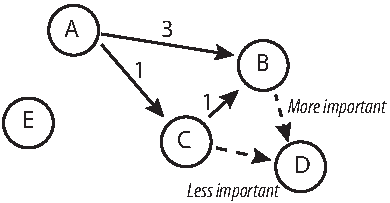
\includegraphics[width=1.0\textwidth]{Figs/forumNetworkExample.pdf}
       \caption{\textnormal{Example social graph induced by forum posts.}}
       \label{fig:forumGraph}
\end{figure}

Nodes $A$, $B$, $C$, $D$, and $E$ represent students. The link from
$A$ to $B$ is marked with the number $3$, because $A$ commented three
times on one of more of $B$'s posts. The number of outgoing links is
the node's {\em out-degree}. For example, the {\em out-degree} of $A$
is $4$.

The number of incoming links is called the node's {\em
  in-degree}. Node $C$'s in-degree is $1$. Node $E$ has no links
entering or exiting. The respective student has not participated in
the forum.

Analogous to Web pages, each node can be assigned a {\em page
  rank}. The intuition in this context is that student $S_1$'s
presence in the forum is more `important' than student $S_2$'s if the
node representing $S_1$ has higher page rank than the node that
represents $S_2$. In our context the intuition behind page rank is
that a node $N$ is more important (has higher page rank) the more
other important nodes comment on $N$'s posts. Imagine a scenario
in which student $S_1$ posts an interesting question, to which many
students comment with their opinion, creating a long thread. The node
representing $S_1$ would experience an increase of its page rank with
every incoming comment. Node $B$ in Figure~\ref{graphExpl} is an
example for this situation. Its in-degree is $4$. If $B$ were to
comment on one of $D$'s posts, then $D$'s page rank would increase
more than if the low-page-rank node $C$ commented on $D$.

In terms of evaluating a student's participation in the forum, a high
page rank, and high out-degree are positive. Low values are less
positive. We chose these two values because of their relatively
straight-forward meanings when applied to forum posts, and for their
relevance to our goal of identifying potential intervention times.

Some of the fifteen other measures we computed, such as {\em
  betweenness} are meaningful for forum scenarios as well, but their
usefulness depends on one's analysis goals. For example,
\cite{yang2013} include several of those measures for the purpose of
prediction analysis. For evaluation contribution quality the contents
of posts would need to be considered: students who persistently post
irrelevant contents contribute less positively to the forum than
constructively participating students. However, for our purposes the
two measures of page rank and out-degree provide strong enough
signals.

\section{Analysis Procedure}

For each course we identified the top 10\% of forum-contributing
students as measured by their postings across the entire course. For
those students we computed the average of our chosen social graph
measures. This average was computed for each week of each
offering. The results provided a week-by-week time series of postings
and evolving pagerank for these students.

Figure~\ref{fig:cs229OutDeg} shows a typical time series with the sum
of postings (i.e. weighted out degree) on the ordinal, and weeks into
the quarter on the abscissa.
%% \begin{figure}[htp]
%%        \centering
%%        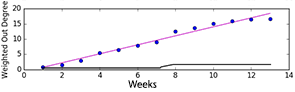
\includegraphics{Figs/comparison_Weighted_Out_Degree_fall16SimplifiedSmall.png}
%%        \caption{\textnormal{Forum post contributions by top 10\% of
%%            contributors throughout an academic quarter (machine learning class).}}
%%        \label{fig:cs229OutDeg}
%% \end{figure}
\begin{figure}[htp]
       \centering
       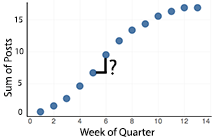
\includegraphics{Figs/CS229Fall14RawDataSmall.png}
       \caption{\textnormal{Page rank by top 10\% of
           contributors throughout an academic quarter (machine learning class).}}
       \label{fig:cs229OutDeg}
\end{figure}
Notice in Figure~\ref{fig:cs229OutDeg} that the successive increases
in average contribution of the top 10\% appear to take a jump after
week 5. Such a discontinuity, or {\em change point} could be a good
trigger for encouragements of students who have held back
participation. However, visual inspection is insufficient for
determining whether this change is statistically significant, or could
easily be explained by random noise instead. The question mark in the
figure is a reminder of this uncertainty.

We therefore next constructed a bootstrapped CUSUM analysis over the
total number of forum posts of a course offering, measured every week
\cite{tayl16}.  For each series of course offerings this analysis
yielded the degree of consistency of significant forum post activity
changes throughout the offerings.

Our bootstrap permuted the post readings, and re-computed the CUSUM
points 1000 times. For each permutation we computed the $S_{diff}^0 =
S_{max}^0-S_{min}^0$ and determined whether $S_{diff}^0$ was less than
the corresponding value $S_{diff}$ in the CUSUMs of the correctly
ordered number of posts. We accepted that a change point occurred
sometime in a quarter at a confidence level of 95\%. That is, we
accepted that a change point occurred if at least 950 of the
permutations yielded an $S_{diff}^0$ less than $S_{diff}$.

Following \cite{tayl16} we determined the last week before a change
for each change point. Figure~\ref{fig:cs229ChangePts} shows an
example.
\begin{figure}[htp]
       \centering
       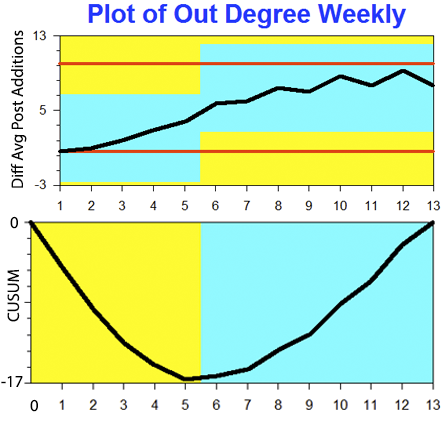
\includegraphics{Figs/cs229Fall14ChangeAnalysis.png}
       \caption{\textnormal{Change points in forum posting 
           time series of a machine learning course.}}
       \label{fig:cs229ChangePts}
\end{figure}
The top chart's line shows changes in the average posts contributions
by the top-10\% contributors during the previous week. The bottom
chart's line shows for each week the accumulated differences from the
mean of the weekly contribution changes. For example, up to about week
five, weekly postings by the top-10\% was below the average of 5. The
corresponding downward segment of the CUSUM reflects increasingly
negative sums of those differences. During week 5 weekly contributions
begin to rise above the mean, and the CUSUM `recovers' upward towards
zero. The left and right blue background bands of
Figure~\ref{fig:cs229ChangePts} (top) are offset between weeks five
and six. The left band covers the ******
[****Explain both the red lines (UCL/LCL) and blue bands.]




%% Figure~\ref{fig:smOutDeg} shows a summary of these series for some of
%% the course offerings. We provide more detailed views further on.
%% \begin{figure}[htp]
%%        \centering
%%        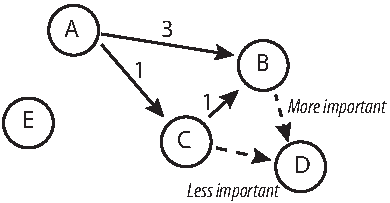
\includegraphics[width=1.0\textwidth]{Figs/forumNetworkExample.pdf}
%%        \caption{\textnormal{Example social graph induced by forum posts.}}
%%        \label{fig:smOutDeg}
%% \end{figure}




\begin{table*}[t]
\centering
\resizebox{\columnwidth}{!}{%
\caption{Summary of Examined Courses}
\label{tab:courseStats}
\begin{tabular}{@{}|>{\columncolor[gray]{0.92}}c|c|c|c|c|c|c|c|c|c|@{}}
\hline
\rowcolor{green!25}
\textbf{Course} & \textbf{Offering} & \textbf{Nodes} & \textbf{Edges}  & \textbf{Contributions}  & \textbf{Density} & \textbf{Active Participants} & \textbf{Largest SCC} & \textbf{Largest WCC} \\ \hline
\textbf{Artificial Intelligence}  & FALL12            & 192            & 414                                & 893  &0.011289267015706806                                            & 106                          & 52                                                    & 105                                                 \\ \hline
                & FALL13            & 278            & 1396           & 4629 &0.018128457522790433                                                                     & 195                          & 130                                                   & 194                                                 \\\hline
                & FALL14            & 435            & 1423                                   & 4352 &0.007537475501880396                                              & 291                          & 149                                                   & 290                                                 \\  \hline
                & FALL15            & 494            & 2114           & 4220 &0.008680227640406993                                         & 357                          & 197                                                   & 352                                                 \\ \hline
                & FALL16            & 782            & 3699           & 7286                                 &0.006056567257532641 &529                          & 332                                                   & 529                                                  \\ \hline
                & SUMMER13          & 137            & 320            & 917 &0.017174753112924                       & 81                           & 39                                                    & 76                                                  \\ \hline 
\textbf{Machine Learning} & FALL11   & 356   & 601   & 1237                          & 0.004755499287862003  & 166                 & 60                                           & 164                                        \\ \hline
               & FALL12   & 581   & 1306  & 2663                        & 0.0038756009258709718 & 283                 & 120                                          & 282                                        \\ \hline
               & FALL13   & 776   & 1823  & 4649                       & 0.003031260392417692  & 383                 & 158                                          & 375                                        \\ \hline
               & FALL14   & 820   & 1943  & 3610                       & 0.002893177283421186  & 449                 & 168                                          & 446                                        \\ \hline
               & FALL15   & 827   & 2413  & 5553                          & 0.0035324153640305545 & 489                 & 219                                          & 489                                        \\ \hline
               & FALL16   & 803   & 1510  & 3140                           & 0.002344698651875914  & 393                 & 153                                          & 386                                        \\ \hline
               & SPRING16 & 331   & 657   & 1548                           & 0.006014831090359792  & 189                 & 65                                           & 
               187      \\ \hline
\textbf{Computer Vision} & FALL11   & 59    & 84    & 248                             & 0.024547048509643482 & 29                  & 12                                           & 29                                         \\ \hline
       & FALL12   & 120   & 195   & 528                            & 0.01365546218487395  & 62                  & 16                                           & 62                                         \\ \hline
       & SPRING16 & 208   & 1018  & 3722                           & 0.023643626904496468 & 150                 & 93                                           & 150                                        \\ \hline
       & WINTER14 & 152   & 601   & 1618                           & 0.026185081910073196 & 101                 & 63                                           & 100                                        \\ \hline
       & WINTER15 & 180   & 702   & 1639                           & 0.021787709497206705 & 125                 & 87                                           & 125                                                                        \\ \hline
\textbf{Decision Analysis} 
                
                  & FALL15   & 176   & 265   & 445                           & 0.008603896103896103 & 100                 & 10                                           & 95                                         \\ \hline
                  & FALL16   & 156   & 373   & 1185                          & 0.015425971877584781 & 104                 & 44                                           & 104  \\ \hline                                     
\textbf{Computational Molecular Biology} & FALL11   & 96    & 348   & 653                            & 0.038157894736842106 & 61                  & 38                                           & 61                                         \\ \hline
                  & FALL12   & 101   & 289   & 657                           & 0.028613861386138615 & 67                  & 41                                           & 67                                         \\ \hline
                  & FALL13   & 123   & 490   & 1279                          & 0.03265360522457684  & 80                  & 52                                           & 80                                         \\ \hline
                  & FALL14   & 140   & 527   & 1122                          & 0.02708119218910586  & 103                 & 66                                           & 103                                        \\ \hline
                  & FALL15   & 147   & 396   & 797                           & 0.018451216102879506 & 93                  & 45                                           & 92                                         \\ \hline
                  & FALL16   & 120   & 384   & 886                           & 0.02689075630252101  & 86                  & 54                                           & 86       \\                                 
\hline

\textbf{International Urbanization Seminar} & FALL14   & 34    & 61    & 419                             & 0.054367201426024955 & 23                  & 9                                            & 23                                         \\ \hline
                    & SPRING14 & 35    & 79    & 379                           & 0.06638655462184874  & 26                  & 8                                            & 26                                         \\ \hline
                    & SUMMER14 & 28    & 67    & 224                             & 0.08862433862433862  & 20                  & 6                                            & 20                                         \\ \hline
                    & FALL15   & 46    & 98    & 352                            & 0.04734299516908213  & 36                  & 19                                           & 36                                         \\ \hline
                    & FALL16   & 44    & 42    & 165                           & 0.022198731501057084 & 31                  & 4                                            & 31                                         \\ \hline
\textbf{Cell and Developmental Biology} & WINTER12 & 214   & 200   & 535                           & 0.004387696897898293  & 65                  & 9                                            & 65                                         \\ \hline
                  & WINTER13 & 157   & 140   & 356                           & 0.0057161522129675    & 55                  & 6                                            & 55                                         \\ \hline
                  & WINTER14 & 140   & 61    & 85                            & 0.0031346351490236382 & 37                  & 1                                            & 35                                         \\ \hline
                  & WINTER15 & 117   & 86    & 135                           & 0.006336575302092543  & 43                  & 5                                            & 43                                         \\ \hline
                  & WINTER16 & 136   & 105   & 297                           & 0.005718954248366013  & 49                  & 3                                            & 49                                         \\ \hline
\textbf{Economic Analysis} & FALL14   & 138   & 80    & 185                            & 0.004231460911879826  & 50                  & 4                                            & 50                                         \\ \hline
                & WINTER15 & 109   & 54    & 142                        & 0.0045871559633027525 & 33                  & 2                                            & 33                                         \\ \hline
                & FALL16   & 217   & 116   & 460                         & 0.002474825055470217  & 65                  & 10                                           & 65                                         \\ \hline
                & SUMMER16 & 12    & 8     & 21                         & 0.06060606060606061   & 5                   & 2                                            & 4                                          \\ \hline
                & WINTER16 & 106   & 74    & 259                         & 0.006648697214734951  & 39                  & 12                                           & 38                                         \\ \hline
\textbf{Indigenous Cultural Heritage} & FALL15   & 11    & 8     & 29                               & 0.07272727272727272 & 5                   & 1                                            & 5                                          \\ \hline
                           & FALL16   & 21    & 47    & 62                              & 0.11190476190476191 & 21                  & 5                                            & 20                                         \\ \hline
\end{tabular}

}
\end{table*}

\begin{figure}[htp]
       \centering
       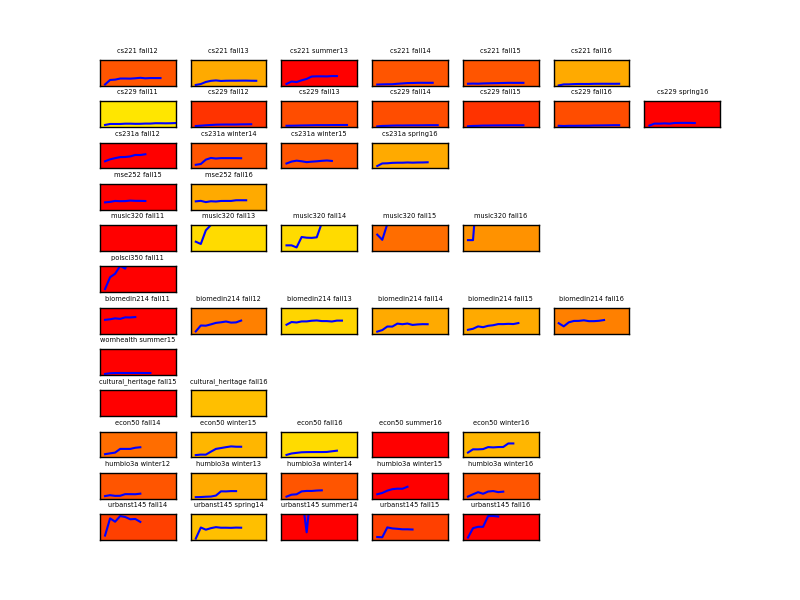
\includegraphics[width=1\textwidth]{Figs/pagerank_sm_color.png}
       \caption{\textnormal{Comparison of Pageranks for top 10\% students}}
       \label{fig:pageRankCompare}
\end{figure}

\begin{figure}[htp]
       \centering
       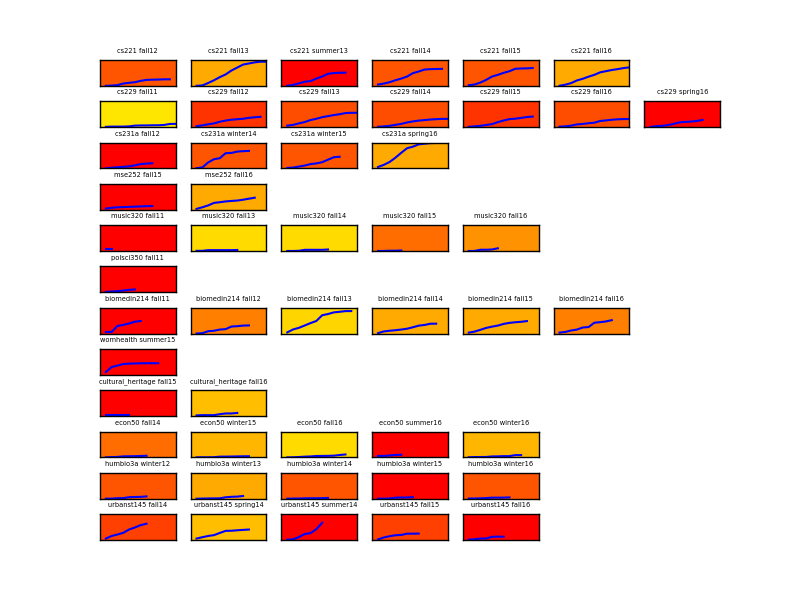
\includegraphics[width=1\textwidth]{Figs/weighted_out_degree_sm_color.png}
       \caption{\textnormal{Comparison of Weighted Out Degrees for top 10\% students}}
       \label{fig:outDegCompare}
\end{figure}

\begin{figure}[htp]
       \centering
       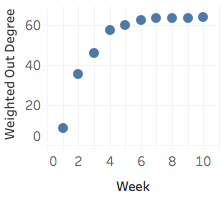
\includegraphics[width=1\textwidth]{Figs/women_health_summer2015_top10.png}
       \caption{\textnormal{A MOOC forum post comparison: Women's
           Global Health.}}
       \label{fig:womenHealth}
\end{figure}


\section{Conclusion and Future Work}

Here is an example chart of the correct size.
\begin{figure}[htp]
       \centering
       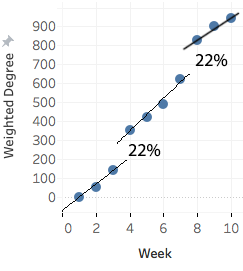
\includegraphics[width=0.5\textwidth]{Figs/exampleChart1.png}
       \caption{\textnormal{Wrong numbers, just an example. See ~/tmp/forumPromptsTableauChartsSample.twb}}
       \label{fig:exampleChart}
\end{figure}


\begin{itemize}
\item Consider student post content quality
\item Consider consistency: contribute throughout course
\item Consider influence on others
\item Draw instructor attention to dense topic clusters, which might
  indicate confusion, or student excitement to harness.
\end{itemize}
%% Control charts are of significance for our scenario, because
%% breakages across control bounds can be observed at any point in
%% time. Instructors could therefore be alerted weekly of any students
%% (or average of larger student groups) who are atypical in their
%% posting behavior. Bootstrap procedures, which permute data points many
%% times, computing target measures like means each time require that all
%% data points are available for the procedure. On the other hand, these
%% procedures can detect multiple change points that occur in the
%% examined data.

